% !TEX program = xelatex
\documentclass[10pt,letterpaper,twocolumn]{article}

\usepackage[top=0.72in,bottom=0.72in,left=0.72in,right=0.72in]{geometry}
\usepackage{fontspec}
\setmainfont{Latin Modern Roman}[
  Extension=.otf,UprightFont=lmroman10-regular,BoldFont=lmroman10-bold,
  ItalicFont=lmroman10-italic,BoldItalicFont=lmroman10-bolditalic]
\setsansfont{Latin Modern Sans}[
  Extension=.otf,UprightFont=lmsans10-regular,BoldFont=lmsans10-bold,
  ItalicFont=lmsans10-oblique,BoldItalicFont=lmsans10-boldoblique]
\setmonofont{Latin Modern Mono}[Extension=.otf,UprightFont=lmmono10-regular,Scale=0.82]
% YWFT Processing is the display face for the title line only: its punctuation
% glyphs are unreliable, so every other run of text on this page is Latin Modern.
\newfontfamily\acbold{ywft-processing-bold}[
  Path=../../system/public/type/webfonts/,Extension=.ttf]

\usepackage{amsmath}
\usepackage{xcolor}
\usepackage{titlesec}
\usepackage{enumitem}
\usepackage{booktabs}
\usepackage{tabularx}
\usepackage{fancyhdr}
\usepackage{hyperref}
\usepackage{xurl}
\usepackage{graphicx}
\usepackage{microtype}
\usepackage{listings}
\usepackage[numbers,sort&compress]{natbib}
\usepackage{tikz}
\usetikzlibrary{arrows.meta,positioning,fit}

\definecolor{acpink}{RGB}{180,72,135}
\definecolor{acblue}{RGB}{44,92,188}
\definecolor{acred}{RGB}{190,48,62}
\definecolor{acdark}{RGB}{48,43,56}
\definecolor{acgray}{RGB}{105,105,110}
\definecolor{aclightgray}{RGB}{244,243,246}

\hypersetup{colorlinks=true,linkcolor=acblue,urlcolor=acblue,citecolor=acblue,
  pdfauthor={@jeffrey},
  pdftitle={Take the Psychology Out of Posting: the oskiewar Reel Factory}}
\titleformat{\section}{\normalfont\bfseries\normalsize\uppercase}{\thesection.}{0.45em}{}
\titlespacing{\section}{0pt}{1.15em}{0.3em}
\titleformat{\subsection}{\normalfont\bfseries\small}{\thesubsection}{0.45em}{}
\titlespacing{\subsection}{0pt}{0.8em}{0.2em}
\pagestyle{fancy}
\fancyhf{}
\renewcommand{\headrulewidth}{0pt}
\fancyhead[C]{\footnotesize\color{acpink}\textit{oskiewar --- the reel factory}}
\fancyfoot[C]{\footnotesize\thepage}
\setlist[itemize]{nosep,leftmargin=1.2em,itemsep=0.1em}
\setlength{\columnsep}{1.7em}
\setlength{\parindent}{1em}
\setlength{\parskip}{0.2em}
\makeatletter
\setlength{\@fptop}{0pt}
\setlength{\@dblfptop}{0pt}
\makeatother
% Tall evidence tables must land near their discussion, not on a float page
% after the bibliography. Loosen the default area fractions accordingly.
\renewcommand{\topfraction}{0.92}
\renewcommand{\dbltopfraction}{0.92}
\renewcommand{\bottomfraction}{0.9}
\renewcommand{\textfraction}{0.06}
\renewcommand{\floatpagefraction}{0.72}
\renewcommand{\dblfloatpagefraction}{0.72}
\setcounter{topnumber}{3}
\setcounter{dbltopnumber}{3}
\setcounter{totalnumber}{4}
\setlength{\textfloatsep}{12pt plus 2pt minus 3pt}
\setlength{\dbltextfloatsep}{12pt plus 2pt minus 3pt}
\setlength{\floatsep}{9pt plus 2pt minus 2pt}
\setlength{\dblfloatsep}{9pt plus 2pt minus 2pt}
\setlength{\abovecaptionskip}{4pt}
% Left-aligned wrapping cells: justified text in a 2in column produces rivers.
\newcolumntype{L}{>{\raggedright\arraybackslash}X}
\newcolumntype{P}[1]{>{\raggedright\arraybackslash}p{#1}}
\tolerance=900
\emergencystretch=1em
\graphicspath{{figures/}{../arxiv-ac/figures/}}
\newcommand{\ac}{\textsc{Aesthetic.Computer}}
\newcommand{\game}{\textsc{oskiewar}}
\newcommand{\code}[1]{\texttt{#1}}
\InputIfFileExists{version.tex}{}{%
  \providecommand{\paperhash}{dev}\providecommand{\paperrev}{?}}

\lstset{basicstyle=\ttfamily\footnotesize,breaklines=true,frame=single,
  rulecolor=\color{acgray!30},backgroundcolor=\color{aclightgray},
  xleftmargin=0.4em,xrightmargin=0.4em,aboveskip=0.5em,belowskip=0.5em}

\begin{document}

\twocolumn[{%
\begin{center}

\includegraphics[height=3.5em]{pals}\par\vspace{0.45em}
{\acbold\fontsize{23pt}{27pt}\selectfont\color{acdark} Take the Psychology Out of Posting}\par
\vspace{0.2em}
{\normalfont\fontsize{12pt}{14pt}\selectfont\color{acpink}
  A Marketing Output Function for \textsc{@oskiewar}\\
  Four Stages from a Date to a Finished Instagram Reel}\par
\vspace{0.55em}
{\normalsize\href{https://prompt.ac/@jeffrey}{@jeffrey}}\par
{\small\color{acgray} Aesthetic.Computer --- 8 August 2026}\par
{\small\color{acgray} ORCID: \href{https://orcid.org/0009-0007-4460-4913}{0009-0007-4460-4913}}\par
\vspace{0.35em}
{\small\color{acblue}\url{https://aesthetic.computer}}\par
\vspace{0.55em}\rule{\textwidth}{1.5pt}\vspace{0.35em}
\end{center}

\begin{quote}
\small\noindent\textbf{Abstract.}
A social account for a game is normally a person deciding, daily, what is worth
showing. This report describes and measures the replacement: a four-stage
function that takes a date and returns a finished, spec-checked 1080$\times$1920
Instagram Reel with nobody choosing anything. Source turns the date into a slot
number and the slot number into a market segment and a seed, by arithmetic.
Render drives the real game in headless Chrome and records the real screen and
the real synthesized audio. Dress writes only words --- caption, tags, cover,
and a conformance check against Meta's published Reels table. Publish is a dry
run that prints the exact bytes it would send. Three reels built on this machine
on 8--9 August 2026 pass all ten checks the file can answer, at 2.4--2.8$\times$
realtime, 94--111 seconds of wall clock apiece. Two results are negative and are
reported as such. First, a seed reproduces a match's \emph{identity} --- the
same string produced match \code{ow-chetty900} on three separate runs --- but
not its frames, because the browser advances the simulation on the wall clock
and tick alignment jitters between runs; the copy in the pipeline is written to
claim only the first, and should not be upgraded. Second, inspection of the
finished files contradicts the pipeline's own account of itself in three places:
every reel opens on roughly 2.7 seconds of the \emph{previous} round's result
card and closes on roughly 0.6 seconds of the \emph{next} round's intro; the
cover frame is sampled at a fixed six seconds and therefore lands, in all three,
on two motionless figures during the countdown; and two of the three carry about
19 seconds of near-silence, with AAC tracks at 21.7 and 22.2 kbps against the
128 kbps Meta's table names and the spec check does not read. Two defects in the
game were found and one was fixed: \code{saveReplay} posts to an absolute
production URL, so every marketing render was filing bot-versus-bot sparring
into the live replay store next to matches real people played, now intercepted
by rewriting \code{fetch} in the page; and \code{matchWins = 5} is never
accumulated, so a ``match'' is one round today. Platform behaviour is cited only
from Meta-owned pages read on 8 August 2026, including a contradiction Meta has
not resolved --- the content-publishing guide says 100 API-published posts per
24 hours and the \code{content\_publishing\_limit} reference says 50 --- which
is quoted rather than settled. The principal limitation is blunt: stage four has
never been run. The \textsc{@oskiewar} account does not exist, so
\code{uploadPublic}, \code{publishLive}, \code{remainingQuota}, and
\code{pullInsights} have been written and read and never executed against the
live API.
\end{quote}
\vspace{0.4em}
}]

\section{The Ask}

\game{} is a two-player fighting game that runs in a browser, on an Xbox in
Developer Mode, and nowhere a stranger can find it \cite{scudder2026oskiewar,
scudder2026store}. The gap between ``it works'' and ``someone plays it'' is
distribution, and on a phone in 2026 distribution means short vertical video.

The usual way to close that gap is a person: someone plays, notices a good
moment, clips it, writes something, posts it. That person has taste, and taste
is the problem. Taste is expensive, it is not available daily, and --- for a
solo developer who would rather be writing the game --- it silently converts
into not posting at all. The instruction that produced this system was to take
the psychology out of it: make posting an output function, not a decision.

An output function has a hard property. Given a date, it returns an artifact,
and if it returns nothing that is a bug rather than a mood. The operator's job
shrinks to watching three videos and saying yes. This report describes the four
stages that function is built from, measures three reels it produced, checks
what it claims against what the files actually contain, and establishes from
Meta's own documentation what the last stage will meet when it is finally
allowed to run.

\section{Method and Evidence}

Three bodies of evidence, and one exclusion.

The code is the repository working tree at commit \code{daf4372f1}
\cite{acrepo}: \code{xbox/live/marketing/} --- \code{source.mjs} (93 lines),
\code{render.mjs} (367), \code{dress.mjs} (73), \code{publish.mjs} (209),
\code{segments.mjs} (129), \code{shell.mjs} (135), \code{reel.mjs} (153) --- plus
\code{xbox/live/hello.js} (6,404 lines) and \code{xbox/live/mac-test.html}
(1,027). Claims about behaviour are grep-checked against that source. Where the
operator's manual \cite{acmarketing} and the source disagree, the source wins
and the divergence is stated.

The artifacts are the three reels staged in
\code{tmp/\allowbreak oskiewar-reels/\allowbreak queue/} on 9 August 2026 (UTC): slots 660, 661, and
662, at \code{2026-08-09-s0-fgc}, \code{-s1-gamedev}, and \code{-s2-retro}. Each
directory holds \code{reel.mp4}, \code{cover.jpg},
\code{thumbnail-10-percent.jpg}, a \code{reel.json} sidecar carrying the render
log and the spec table, and the raw frame directory and per-frame concat list
the encoder was driven from. Every number in \S\ref{sec:throughput} and
\S\ref{sec:artifacts} was measured from those files with \code{ffprobe} and
\code{ffmpeg} \cite{ffmpeg} at the time of writing, not copied out of a prior
session's log. Where a figure comes from the operator's own run rather than from
a file I could re-measure --- the determinism experiment in
\S\ref{sec:determinism} is the whole of that category --- it is labelled.

The platform side is Meta-owned pages only, eight of them, each fetched and read
in full on 8 August 2026 and listed in the bibliography with that access date.
The exclusion: no third-party summary, SMM-vendor blog, or forum answer is used
as evidence anywhere in this paper, and where Meta's pages contradict each other
the contradiction is quoted rather than arbitrated.

\section{Stage 1 --- Source: Arithmetic Instead of Taste}

The first stage is the whole thesis in fifty lines. A date and an index become
an absolute slot number,
\[
\text{slot} = \text{days since 2026-01-01} \times \text{slots per day} + \text{index},
\]
and everything downstream is a pure function of that integer. The slot indexes a
fixed ten-entry rotation to pick a market (Table~\ref{tab:rotation}). The seed
string is \code{YYYY-MM-DD\#index}, hashed with FNV-1a into the 32-bit value the
renderer seeds the simulation with. Slot zero is pinned to 1 January 2026 and
documented as unmovable, because moving it would renumber every past post and
silently reshuffle which market owns which slot.

\begin{table}[!t]
\centering
\caption{The market rotation, read from \code{segments.mjs}. Ten slots, so a
share is legible at a glance: a fighting game lands hardest in the FGC, and the
other four markets exist to keep the account from reading as a single note.
Changing the \code{rotation} array is the only supported way to change the mix.}
\label{tab:rotation}
\footnotesize
\begin{tabularx}{\columnwidth}{@{}P{0.13\columnwidth}P{0.16\columnwidth}P{0.07\columnwidth}L@{}}
\toprule
Key & Market & Share & What it is told to say \\
\midrule
\code{fgc} & fighting game & 3/10 & hitboxes, hitstun, grabs, a ball nobody asked for \\
\code{gamedev} & indie gamedev & 2/10 & no engine, one file, fixed timestep, headless tests \\
\code{retro} & pixel + arcade & 2/10 & drawn with lines at runtime, no sprites, arcade rules \\
\code{gen} & generative art & 2/10 & the date seeds the match; the audio is synthesized live \\
\code{homebrew} & console homebrew & 1/10 & same source on console under JavaScriptCore, no port \\
\bottomrule
\end{tabularx}
\end{table}

One slot in five --- those with $\text{slot} \bmod 5 = 4$ --- is supposed to
pull a real recorded round out of \code{/api/oskiewar-replays} instead of
generating a synthetic one, so the feed is not only robots sparring. Which round
is still arithmetic: the store is asked for its recent rounds, anything under
seven seconds of play is dropped as a whiff rather than a fight, and the seed
indexes what is left. If the store is unreachable the stage falls back to
self-play and says so in the log. None of the three staged slots satisfies
$\text{slot} \bmod 5 = 4$, so this branch was not exercised; when I queried the
endpoint on 8 August 2026 it returned an authentication error, which means the
fallback --- not the replay lane --- is what would run today.

The seed works at all because of a property of the game rather than of the
factory. \code{hello.js} calls \code{Math.random} exactly once, at line 611, to
seed the match-name generator; ball kind, round names, and the fighters all fall
out of that one draw. Replacing \code{Math.random} with a seeded generator
before the page boots therefore fixes the identity of the entire match from a
string. A code comment at line 1649 records that this was not always true: an
earlier version drew ball radius and mass from \code{Math.random} directly,
``which silently made ball radius and mass unreproducible.''

\section{Stage 2 --- Render: the Real Game, at the Real Shape}

Stage two runs \code{mac-test.html} and \code{hello.js} in headless Chrome
through the same frame driver a player gets, served by a small local shell
(\code{shell.mjs}) that lists every module the page imports. Video and audio are
captured by two separate mechanisms, both borrowed from the sibling
\code{marketing/av-reels} lane \cite{acavreels}.

Video is the Chrome DevTools Protocol \code{Page.\allowbreak start\-Screen\-cast} domain
\cite{cdp}: a JPEG frame arrives whenever the page repaints, carrying a
timestamp. The handler writes each frame to disk with its arrival time and the
encoder is later driven from a concat list with per-frame durations, so a
dropped repaint stretches its own frame instead of speeding up the whole reel.
Measured across the three staged reels, the median inter-frame gap is
16.70\,ms in all three --- one 60\,Hz repaint, exactly --- with 4, 1, and 0 gaps
longer than 33\,ms and worst cases of 80.0, 71.9, and 33.3\,ms. That is a clean
capture: the pacing artifact the concat list exists to absorb barely occurs.

Audio cannot be captured the same way, because headless Chrome throttles
\code{requestAnimationFrame} and leaves \code{canvas.captureStream()} empty. The
established \ac{} technique is to patch \code{AudioNode.prototype.connect}
before the page boots, so that anything a node routes to \code{ctx.destination}
is additionally routed to a \code{MediaStreamDestination} that an in-page
\code{MediaRecorder} is listening to. Audio worklets run on the audio thread,
which is why this survives the throttle. There is no second audio path in the
system; the reel either carries the game's own synthesis or it carries nothing.

\begin{figure}[!t]
\centering
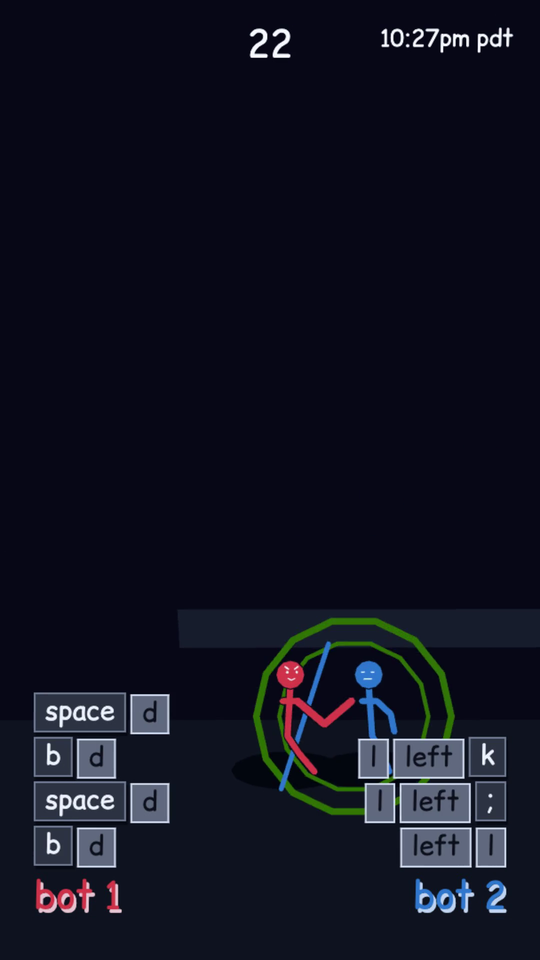
\includegraphics[width=0.46\columnwidth]{reel-frame}
\caption{One frame of a finished reel, 14 seconds into slot 660, at the native
capture size of 1080$\times$1920 and untouched afterwards. The reel is recorded
at 9{:}16 rather than cropped into it, and the argument for doing so is visible
here as a cost as well as a benefit: the game lays itself out for the viewport
it is handed and keeps the camera on the ground plane, so the fight --- the
green impact ring, the two figures, the keycap legends, the handles --- lives in
the bottom third and the top half is empty sky. Nothing is composed on top of
this, which is the point; but nothing fills the space either.}
\label{fig:frame}
\end{figure}

Capture is 1080$\times$1920 natively. The game is handed a 9{:}16 viewport and
goes compact on its own, so the reel is the real thing at the real shape
(Figure~\ref{fig:frame}). Three things the renderer deliberately cuts: the live
spectator WebSocket is stubbed, because a marketing render is not a match anyone
should be able to walk in on --- and stubbing it roughly halved render time;
replay POSTs are redirected to the local shell (\S\ref{sec:bugs}); and the debug
hitboxes that used to flash on every impact for every player are now gated
behind a view mode, so ordinary play, and every recording of it, is clean.

\section{Stage 3 --- Dress: the Words, and Only the Words}

Nothing is drawn on the video. No plate, no bands, no blurred backdrop, no
burned-in type. What survives in stage three is the part that was never pixels:
one line of copy, one line of address, nine hashtags, a cover frame, a review
thumbnail, and a conformance check.

The caption budget is deliberately under the ceiling. Meta allows 2,200
characters and 30 hashtags \cite{metaPublishing}; the staged captions run
181--300 characters and 8--9 tags, because a keyword dump is not a post. The
check is the interesting part: \code{inspect()} reads the finished file with
\code{ffprobe} and answers, from the file itself, every row of Meta's Reels
specification table that a file can answer, then fails the build loudly if any
row fails (Table~\ref{tab:spec}).

One row is a self-imposed tripwire rather than a platform requirement. Meta
accepts any aspect between 0.01{:}1 and 10{:}1 and merely recommends 9{:}16
\cite{metaMedia}; \code{inspect()} requires 9{:}16 to within $10^{-3}$. The
reason is historical and is worth keeping: an earlier version of this pipeline
captured the game at 1{:}1 and composed the square into a 9{:}16 letterbox with
a blurred backdrop and burned-in type. That design was rejected in favour of
native capture, and the aspect check is the guard that keeps it rejected --- a
drift off 9{:}16 now means something rescaled the video, which is the one thing
this stage must never do.

\begin{table}[!t]
\centering
\caption{Conformance against Meta's published Reels specification
\cite{metaMedia}. The first ten rows are what \code{inspect()} checks; measured
values are from \code{ffprobe} on the three staged files. The last five rows are
requirements the check does not read --- four hold anyway, and one does not.}
\label{tab:spec}
\footnotesize
\begin{tabularx}{\columnwidth}{@{}P{0.20\columnwidth}P{0.24\columnwidth}L@{}}
\toprule
Requirement & Meta's value & Measured (slots 660/661/662) \\
\midrule
Container & MOV or MP4 & \code{mp4} \\
Video codec & HEVC or H264 & \code{h264} High \\
Audio codec & AAC & \code{aac} LC \\
Sample rate & $\leq$48\,kHz & 48\,000\,Hz \\
Channels & 1 or 2 & 2 \\
Frame rate & 23--60 fps & 30.00 \\
Max width & $\leq$1920\,px & 1080\,px \\
Aspect & 0.01{:}1--10{:}1 & 0.5625 (9{:}16) \\
Duration & 3\,s--15\,min & 39.55 / 39.60 / 39.60\,s \\
File size & $\leq$300\,MB & 7.03 / 3.19 / 2.94\,MB \\
\midrule
\code{moov} first & required & \code{moov} before \code{mdat} \\
Scan & progressive & \code{progressive} \\
Chroma & 4:2:0 & 4:2:0 (full-range tag) \\
Video rate & VBR, $\leq$25\,Mbps & 1.29 / 0.62 / 0.56\,Mbps \\
Audio rate & 128\,kbps & \textbf{121.5 / 21.7 / 22.2\,kbps} \\
\bottomrule
\end{tabularx}
\end{table}

\section{Stage 4 --- Publish: Dry by Default}

The last stage writes \code{payload.json}: the exact container body, the
status-poll URL, and the publish call it would send. Nothing leaves the machine.
Adding \code{--live} uploads the mp4 and the cover to a public bucket --- Meta
fetches \code{video\_url} itself, so it has to be reachable without
authentication --- reads the account's remaining quota, refuses to post if the
quota is spent, runs the three-call sequence, and appends to a ledger. The
ledger records segment, seed, slot, kind, round, timestamp, and media id, which
is the entire reason a market segment is recorded at all: without it, per-market
performance is unknowable and the rotation in Table~\ref{tab:rotation} can never
be corrected by evidence.

The one hard rule in this stage is negative. Publishing goes through the
official content-publishing endpoints only: no \code{instagrapi}, no session
cookies, no scripted app login. That road has been walked in this repository
before, on \textsc{@whistlegraph}, and it ended in a \code{login\_required} and a
defensively soft-locked account during a 2026 account-integrity ban wave
\cite{acgridpruning}. \code{publish.mjs} contains no other path and should not
grow one.

\section{What a Seed Buys, and What It Does Not}
\label{sec:determinism}

The pipeline's most attractive claim is also the one most likely to be
overstated, so it was tested and the result is partly negative
(Table~\ref{tab:determinism}).

\begin{table}[!t]
\centering
\caption{The determinism experiment, run by the operator on 8--9 August 2026
with seed \code{2026-08-09\#1}. Match identity reproduced across three runs;
frames did not. This is the boundary the copy in \code{segments.mjs} is written
to respect.}
\label{tab:determinism}
\footnotesize
\begin{tabularx}{\columnwidth}{@{}P{0.25\columnwidth}P{0.10\columnwidth}L@{}}
\toprule
Property & Same? & Evidence \\
\midrule
Match name & yes & \code{ow-chetty900} on all three runs \\
Ball kind, fighters & yes & downstream of the single \code{Math.random} draw \\
Frame bytes & \textbf{no} & MD5 of the frame at $t=8$\,s differs between two runs \\
Round outcome & untested & only identity and frames were compared \\
\bottomrule
\end{tabularx}
\end{table}

The cause is structural rather than incidental. The renderer seeds
\code{Math.random} but does not take over the clock: the browser advances the
simulation on wall time, so the number of ticks that elapse between two
particular repaints differs between runs, and the frames drift out of alignment
even though every random draw is identical. A seed therefore reproduces
\emph{which match this is} --- its name, its ball, its fighters, and so its
addressable replay --- and not \emph{what it looked like}.

That is the honest statement, and it is the one the marketing copy makes. The
segment captions say the date names the match and picks the ball; none of them
claims frame-identical reproduction. The temptation to upgrade the claim to
``same seed, same frames'' should be resisted until the renderer is moved onto a
fixed timestep, at which point the claim would become true and worth making.

This is also the only measurement in the paper I did not take myself: re-running
it requires driving headless Chrome, which the machine this was written on
cannot do concurrently with a LaTeX build. The three staged \code{reel.json}
files are consistent with it --- slot 661, seeded \code{2026-08-09\#1}, records
\code{ow-chetty900} as the first match it observed --- but a single consistent
sidecar is corroboration, not replication.

\section{Throughput}
\label{sec:throughput}

Table~\ref{tab:throughput} is the cost of a day's output, measured rather than
estimated. Three reels, built back to back on one M-series laptop with nothing
else running, cost 304.5 seconds of wall clock and produced 118.75 seconds of
finished video: 2.56$\times$ realtime overall, 2.38--2.80$\times$ per reel.

\begin{table}[!t]
\centering
\caption{Per-reel throughput, from the \code{render} block of each
\code{reel.json} and from the per-frame concat lists. Slots 660, 661, and 662
are the \code{fgc}, \code{gamedev}, and \code{retro} markets. ``Capture rate'' is
captured frames divided by the span they cover; the output is re-timed to a
constant 30\,fps at encode.}
\label{tab:throughput}
\footnotesize
\begin{tabularx}{\columnwidth}{@{}P{0.06\columnwidth}P{0.10\columnwidth}P{0.09\columnwidth}P{0.11\columnwidth}P{0.12\columnwidth}L@{}}
\toprule
Slot & Wall & Frames & Capture & Reel & Size / ratio \\
\midrule
660 & 110.6\,s & 2{,}365 & 59.8\,fps & 39.55\,s & 7.03\,MB, 2.80$\times$ \\
661 & 99.6\,s & 2{,}374 & 59.9\,fps & 39.60\,s & 3.19\,MB, 2.52$\times$ \\
662 & 94.3\,s & 2{,}377 & 60.0\,fps & 39.60\,s & 2.94\,MB, 2.38$\times$ \\
\midrule
total & 304.5\,s & 7{,}116 & --- & 118.75\,s & 13.2\,MB, 2.56$\times$ \\
\bottomrule
\end{tabularx}
\end{table}

Three slots a day is therefore about five minutes of machine time, which fits in
the gap between two builds and is nowhere near any published ceiling: at three
posts a day the grid could triple before Meta's post cap is the binding
constraint, on either reading of that cap (\S\ref{sec:platform}). The wall-clock
figure is dominated by something other than encoding, and it is worth naming:
the renderer waits out whatever round was already in progress when the page
opened before it starts recording, so roughly half of each reel's wall clock is
a warm-up round nobody will ever see. That is the price of wanting to start on a
round boundary --- and, as \S\ref{sec:artifacts} shows, it is currently being
paid without the boundary being hit.

\section{What the Artifacts Actually Show}
\label{sec:artifacts}

A pipeline that reports its own success is not evidence. The three finished
files were inspected directly, and they disagree with the pipeline's account of
itself in three places. All three findings are content and timing defects rather
than crashes, which is exactly the class of failure an automated poster is most
likely to ship.

\subsection{The reel does not start where the code says it does}

\begin{figure*}[!t]
\centering
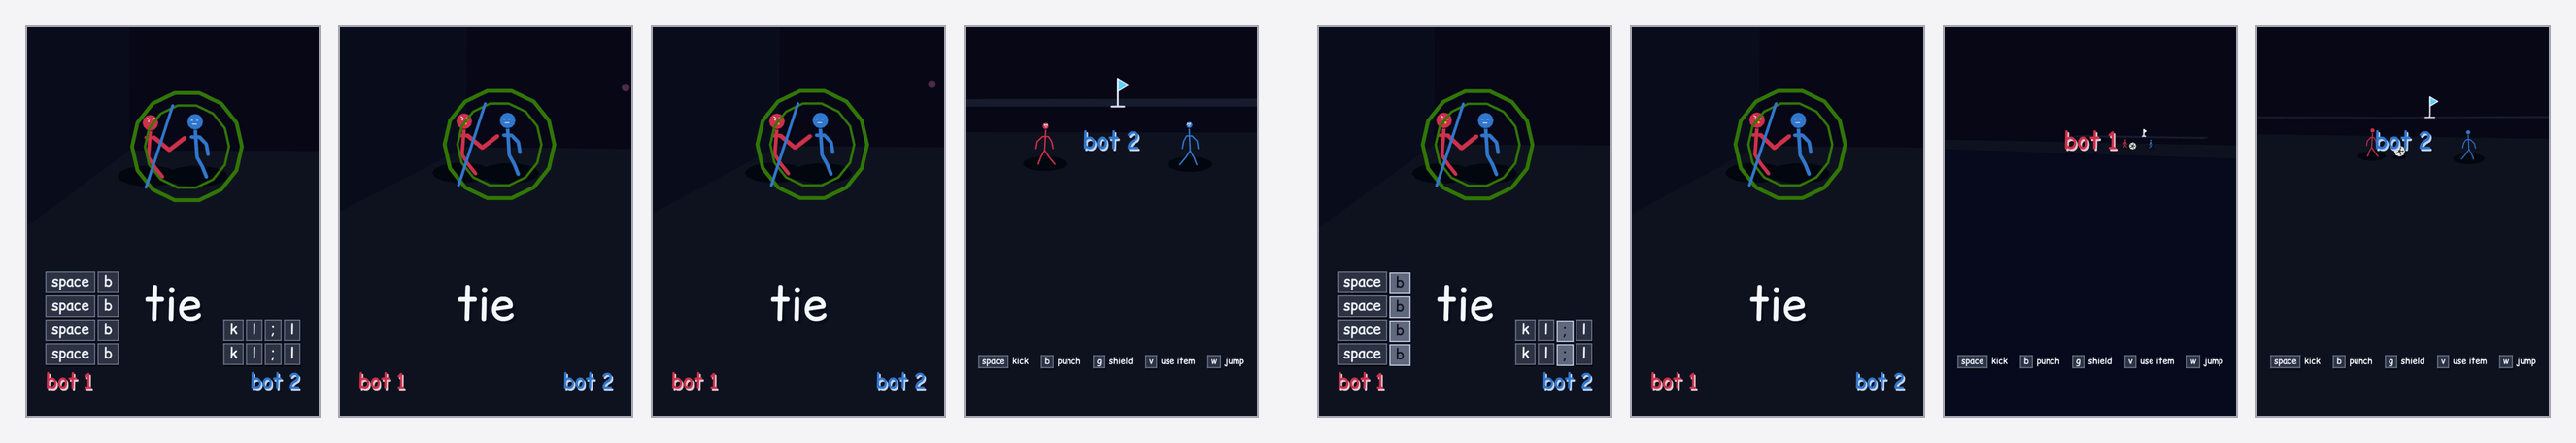
\includegraphics[width=\textwidth]{trim}
\caption{Where slot 660 actually begins and ends. Frames are cropped to the
bottom three-quarters, because the top quarter is empty in every one of them.
Left group, at $t=0.30$, 1.60, 2.60, and 3.60\,s: the reel opens on the tail of
the \emph{previous} round's result card --- ``tie'', two figures inside a green
impact ring --- and only cuts to the recorded round's own intro between 2.65 and
2.78\,s. Right group, at $t=36.60$, 38.60, 39.10, and 39.45\,s: the recorded
round's result card gives way, about 0.65\,s before the end, to the intro of the
round after it. All three staged reels behave identically. The cause is in the
signal, not the timing: a round announces its end by POSTing its replay, which
happens \emph{before} the result card clears, so ``wait for the previous round
to end'' lands in the middle of the previous round's ending.}
\label{fig:trim}
\end{figure*}

\code{render.mjs} waits for the shell to observe a completed round before it
starts the screencast, and its comment says this makes recording ``begin on a
round's own first frame.'' It does not. Figure~\ref{fig:trim} shows the head and
tail of slot 660: the reel opens with about 2.7 seconds of the previous round's
result card and ends with about 0.6 seconds of the next round's intro. Slots 661
and 662 cut at 2.9 and 2.9 seconds respectively. Roughly 3.3 seconds of a
39.6-second reel --- 8\% --- is a neighbouring round.

The mechanism is a signal that fires early. A round ends by POSTing its replay,
and the result card holds for a further 3.6 seconds after that; the renderer
treats the POST as the boundary, so it starts recording 3.6 seconds before the
new round begins and stops 3.6 seconds after the recorded one ends --- which is
just long enough for the round after to start. The fix is not a longer wait but
a different signal, or a fixed offset applied to the one that exists.

\subsection{The cover frame lands on nothing happening}

\begin{figure}[!t]
\centering
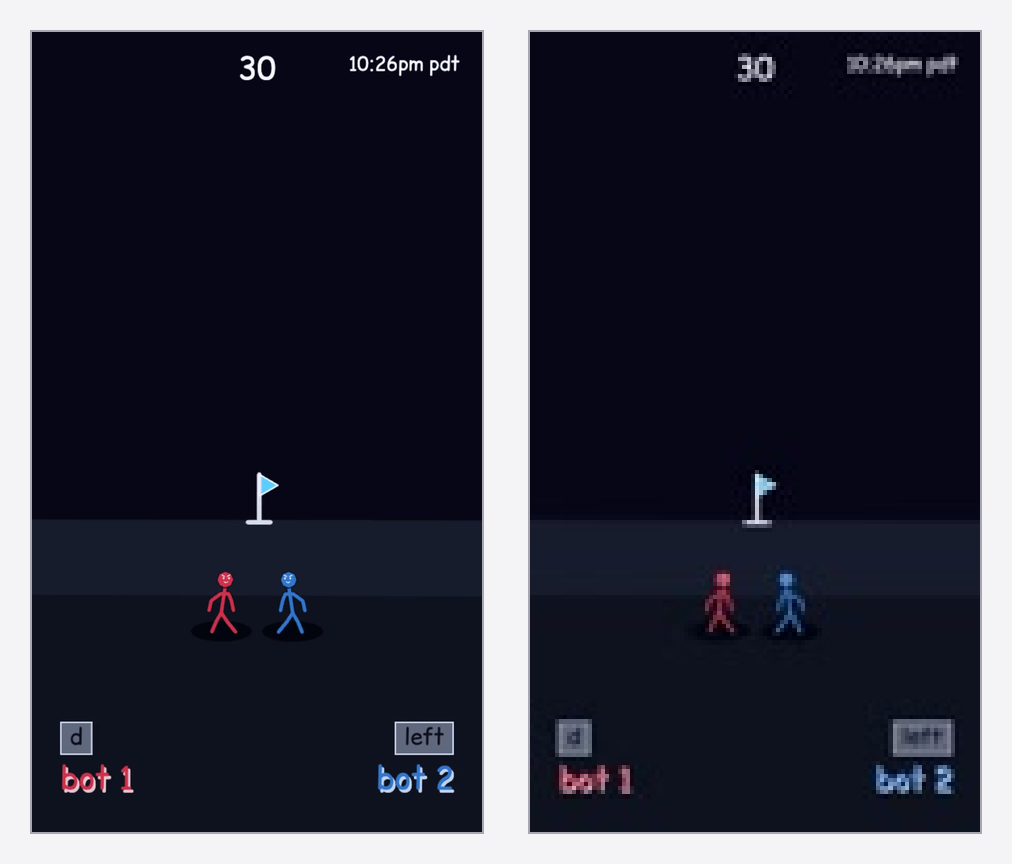
\includegraphics[width=\columnwidth]{slidecop}
\caption{The Slidecop test \cite{acscore}, run rather than asserted. Left: the
cover frame \code{dress.mjs} chose for slot 660 --- the frame Meta will use as
the poster in a feed. Right: the same frame rebuilt from the 108$\times$192
pixels of the review thumbnail written beside it, which is 1\% of the data and
about the size the image gets in a phone's grid. With no burned-in type left to
read, the test now asks whether the \emph{fight} survives the shrink. It does
not, and the reason is not resolution: the fixed six-second cover offset,
displaced by the 2.7\,s of leading result card in Figure~\ref{fig:trim}, lands
3.3\,s into a round that has not started fighting yet. Two motionless figures,
an empty sky, and a flag.}
\label{fig:slidecop}
\end{figure}

\code{dress.mjs} samples the cover at a fixed six seconds, ``past the intro
count.'' Given the leading result card, six seconds is only about 3.3 seconds
into the recorded round, which is still the countdown. In all three staged reels
the cover shows two stick figures standing still. Figure~\ref{fig:slidecop} runs
the house Slidecop check on it: at the tenth-scale the review thumbnail
reproduces, there is no fight to read, and the frame the system would hand Meta
as its poster is the least interesting one in the file. The check is doing its
job --- it produced the thumbnail that reveals this --- but nothing in the
pipeline reads its own output and fails on it, so the poster ships.

\subsection{Two of three reels are mostly silent}

The audio tee works: all three reels carry a real AAC track at 48\,kHz, stereo,
at mean levels of $-22.5$, $-24.2$, and $-23.7$\,dBFS with peaks at $-0.9$,
$0.0$, and $-0.6$\,dBFS --- healthy headroom, no clipping to speak of. What is
in the track is another matter. Silence detection at $-70$\,dB finds, in slots
661 and 662, two dead stretches of 8.93 and 9.72 seconds back to back, from
about 6.9\,s to 25.9\,s: roughly 19 seconds of a 39.6-second reel with nothing
audible in it. Slot 660 has no such gap.

The corresponding numbers are in the last row of Table~\ref{tab:spec}. The AAC
tracks of the two quiet reels average 21.7 and 22.2\,kbps against the 128\,kbps
\code{ffmpeg} was asked for and the 128\,kbps Meta's own table names, and carry
1,143 and 1,051 frames where a gapless 39.6-second stream at 48\,kHz would carry
about 1,856. The recorder emits nothing while nothing is audible, and the gaps
survive into the container.

This is not a bug in the capture. It is the content: in those two rounds the
self-play bots never closed distance, so there were no impacts to synthesize.
Which is the finding that matters most for an automated poster --- the machinery
is sound and the material is thin. All three staged rounds also end in a tie,
which is a weak ending three times out of three. A function that reliably
returns a technically conformant video of two robots not fighting has solved the
posting problem and not the marketing problem.

\section{Two Findings in the Game}
\label{sec:bugs}

Building the factory surfaced two facts about \game{} itself that had nothing to
do with marketing.

\subsection{Every render was polluting the production replay store}

\code{saveReplay} in \code{mac-test.html} posts to
\url{https://aesthetic.computer/api/oskiewar-replays} --- an \emph{absolute}
production URL. A local shell therefore cannot intercept it by serving that
path, which is the obvious and wrong assumption. Until this was found, every
marketing render filed its bot-versus-bot sparring into the live replay store,
next to matches real people played, at a rate of two to three rounds per reel.
The staged sidecars record exactly that count under
\code{replayPostsSwallowed}: 3, 2, and 2.

The fix is in \code{render.mjs}, in the pre-boot script: \code{globalThis.fetch}
is rewritten so that any request whose URL contains
\code{/api/oskiewar-replays} is reissued against the local origin as a bare
path. The rewrite does double duty --- it protects the store, and because the
local shell now receives every replay POST, it is also how the factory learns
that a round has just ended.

The general lesson is worth stating separately from the fix. A page that hard-codes
its own production origin cannot be sandboxed by controlling the server; it has
to be sandboxed by controlling the client. Anything in \ac{} that a headless
harness might one day drive should be reachable by relative path, and where it
is not, the harness must rewrite \code{fetch} rather than assume a local server
is enough.

\subsection{A match is a round}

\code{hello.js} declares \code{matchWins = 5} and the result screen prints it,
but nothing accumulates round wins toward it: self-play calls
\code{startSelfPlay} again at every round end, and normal play returns to the
title. The replay store agrees --- the operator's audit found all 464 stored
rounds carrying \code{roundIndex: 0}. So a ``full match'' today is one round:
intro countdown, fight, KO or time-out, result card.

The factory is written to survive that being fixed rather than to depend on it:
\code{renderReel} takes a \code{rounds} count and already records more than one
if asked. But the honest description of what these reels contain is one round,
and the operator's manual is right to say so in a block quote rather than to let
``a whole match, uncut'' stand unqualified. I could not re-verify the 464 figure
myself: the public replay endpoint returned an authentication error when queried
on 8 August 2026.

\section{The Platform}
\label{sec:platform}

Everything in this section is from Meta-owned pages read on 8 August 2026. It is
recorded here because stage four has never run, so the documentation is
currently the only thing standing between the payload and a real post.

\subsection{The route, and what it does not require}

\game{} would publish through the Instagram API with Instagram Login, on
\code{graph.instagram.com}. Two properties of that route matter for a solo
developer. First, no Facebook Page: ``This API setup does not require a Facebook
Page to be linked to the Instagram professional account'' \cite{metaIgLogin} ---
one fewer entity to own and keep alive. Second, no review: Standard Access is
the default level, and ``If your app only serves your Instagram professional
account or an account you manage, Standard Access is all your app needs''
\cite{metaOverview}. Advanced Access, which does require App Review and Business
Verification, is only ``required if your app serves Instagram professional
accounts that you don't own or manage'' \cite{metaOverview}. Publishing to your
own account is therefore a same-day setup, and the scopes are
\code{instagram\_business\_basic} and
\code{instagram\_business\_content\_publish} \cite{metaPublishing,metaIgLogin}.
The account itself must be a professional (business or creator) account
\cite{metaOverview}; the API cannot touch a consumer account.

\subsection{Three calls, and a container that expires}

Publishing is three calls \cite{metaPublishing}. \code{POST /\{ig-user-id\}/media}
creates a container, with \code{media\_type=REELS}, a publicly fetchable
\code{video\_url}, a caption, and an optional \code{cover\_url}.
\code{GET /\{container-id\}?fields=status\_code} polls it; Meta's own cadence
advice is exact --- ``We recommend querying a container's status once per
minute, for no more than 5 minutes'' --- and the status vocabulary is
\code{EXPIRED}, \code{ERROR}, \code{FINISHED}, \code{IN\_PROGRESS},
\code{PUBLISHED}, with expiry described as ``The container was not published
within 24 hours and has expired.'' \code{POST /\{ig-user-id\}/media\_publish}
with \code{creation\_id} finishes the job. \code{publish.mjs} implements exactly
this cadence: five polls, one minute apart, then a hard failure on any terminal
state other than \code{FINISHED}.

\subsection{The rate limit Meta has not settled}

Two Meta-owned pages give two different numbers. The content-publishing guide
says: ``Instagram accounts are limited to 100 API-published posts within a
24-hour moving period'' \cite{metaPublishing}. The
\code{content\_publishing\_limit} reference defines \code{quota\_total} as ``The
maximum number of IG Containers the app user can publish within the
\code{quota\_duration} time period (currently 50)'' and its sample response
carries 50 over a \code{quota\_duration} of 86,400 seconds \cite{metaLimit}.

I am not going to resolve that, because I cannot: both pages are live, both are
Meta's, and neither acknowledges the other. The engineering answer is to not
depend on the constant. \code{publish.mjs} reads
\code{content\_publishing\_limit} at runtime and refuses to post when the
account's own reported quota is spent, which is correct under either number. A
third, separate ceiling sits underneath both: ``An Instagram account can only
create 400 containers within a rolling 24 hour period'' \cite{metaMedia}. At
three posts a day none of the three binds, which is why the contradiction is
reportable rather than urgent.

\subsection{Tokens expire on a schedule that needs a calendar}

The token path is a short-lived token from authorization, exchanged at
\code{GET graph.\allowbreak instagram.\allowbreak com/\allowbreak access\_token} with
\code{grant\_type=ig\_exchange\_token} for a long-lived token ``valid for 60
days,'' refreshed at \code{GET graph.\allowbreak instagram.\allowbreak com/\allowbreak refresh\_\allowbreak access\_token} with
\code{grant\_type=ig\_refresh\_token} \cite{metaBusinessLogin}. The refresh has
three preconditions, and the first is the operational one: ``The existing
long-lived access token is at least 24 hours old,'' it must not have expired,
and the app must hold \code{instagram\_business\_basic}. Meta is explicit about
the cliff: ``Tokens that have not been refreshed in 60 days will expire and can
no longer be refreshed'' \cite{metaBusinessLogin}. There is no revival past
that, only a fresh OAuth round-trip. A monthly reminder is part of the system,
not an afterthought.

\subsection{Insights, and the metrics that no longer exist}

Per-market reporting is the reason the ledger records a segment, and it depends
on metrics that Meta has been actively pruning. The changelog entry dated 21
January 2025 deprecates \code{clips\_replays\_count},
\code{ig\_reels\_aggregated\_all\_plays\_count}, \code{impressions} on media and
user insights, and \code{plays} on media insights, ``Applies to v22.0+. Will
apply to all versions April 21, 2025,'' and introduces \code{views} in the same
entry \cite{metaChangelog}. A later entry, 3 December 2025, adds
\code{reels\_skip\_rate} and \code{reposts} \cite{metaChangelog}. The metrics
currently documented for a Reel are \code{views}, \code{reach}, \code{likes},
\code{comments}, \code{saved}, \code{shares}, \code{total\_interactions},
\code{reposts}, \code{reels\_skip\_rate}, \code{ig\_reels\_avg\_watch\_time},
and \code{ig\_reels\_video\_view\_total\_time} \cite{metaInsights}.

Two cautions come with them, both from Meta's own labels. Several of these ---
\code{views}, \code{total\_interactions}, \code{ig\_reels\_video\_view\_total\_time}
--- are flagged ``Metric in development,'' and \code{reach} and
\code{reels\_skip\_rate} are flagged ``estimated'' \cite{metaInsights}. Numbers
carried into the ledger from those fields will drift from the app's own UI, and
a rotation adjusted on small differences between markets would be adjusting on
noise. \code{reels\_skip\_rate}, which measures the share of viewers who left
inside the first three seconds, is the only one of them that judges a hook
directly --- and, given \S\ref{sec:artifacts}, the one this account should read
first.

\section{Ethics, Privacy, and Limits}

\subsection{The private API is not an option}

The rule is absolute and the reason is experience rather than principle. This
repository has a scripted, unofficial Instagram path in its history: an
\code{instagrapi} archive run against \textsc{@whistlegraph} returned
\code{login\_required} and left the session broken, on an account that
Instagram had already soft-locked, during the 2026 account-integrity ban wave
\cite{acgridpruning}. The audit that followed concluded that third-party
mass-action tools log in through the private mobile API and get flagged as bots,
and that the scripted path should not be retried. \code{publish.mjs} therefore
speaks only the documented content-publishing endpoints, and
\code{social/accounts.json} carries that constraint on the
\code{oskiewar-ig} row itself \cite{acsocial} so that it is visible to whoever
next opens the ledger rather than only to whoever reads this paper.

\subsection{Renders must not pollute the record}

The replay store is a record of matches people played. A marketing render is not
one, and the finding in \S\ref{sec:bugs} is that it was being written into that
record anyway. The rule the fix encodes: a synthetic render may read production
state and may never write it. The local shell makes that structural rather than
aspirational --- it accepts every replay POST and stores none of them, and only
proxies GETs to production when a slot is legitimately replaying a real round.
Two consequences follow that are worth stating. Marketing renders should not
appear in any public count of matches played, and the 464-round figure quoted in
\S\ref{sec:bugs} is itself from a store that had been receiving robot rounds,
which is one more reason to treat it as the operator's measurement rather than a
clean census.

\subsection{Nothing auto-posts}

The queue is staged, not scheduled. Building three reels writes three
directories and stops; publishing is a separate command; publishing for real
additionally requires \code{--live} and a token in the environment. The
suggested scheduler in the operator's manual is a single crontab line that
builds and leaves the results staged \cite{acmarketing}, and the manual is
explicit that automating stage four is one line that should be written after a
few weeks of watching what the queue produces, not before. This paper's evidence
argues for keeping it that way somewhat longer than planned: a fully automated
stage four, running today, would have posted three technically conformant videos
whose covers show nobody fighting and two of which are silent for half their
length.

There is a second reason to keep a human in the loop that has nothing to do with
quality. The reels depict only synthetic play by default; the one-in-five replay
slot depicts a round a real person played, addressed by its round name. Those
rounds are already public and addressable \cite{scudder2026url}, and no handle,
face, or private datum is in the frame --- but a system that automatically
promotes a stranger's match to a marketing channel is a different thing from one
that renders robots, and it should not cross that line without someone deciding
that it may.

\subsection{What is not verified}

Stated plainly rather than smoothed over.

\begin{itemize}
  \item \textbf{Every stage-four call.} \code{uploadPublic}, \code{publishLive},
    \code{remainingQuota}, and \code{pullInsights} have never been executed
    against the live API. The \textsc{@oskiewar} account does not exist
    \cite{acsocial}. This is the principal limitation of the whole report: the
    stage with the most external dependencies is the only one with no measured
    behaviour at all.
  \item \textbf{Whether the real post cap is 50 or 100.} Meta contradicts itself
    \cite{metaPublishing,metaLimit}; the endpoint is read at runtime instead.
  \item \textbf{Any byte-range or redirect requirement on \code{video\_url}}
    beyond ``publicly accessible.'' Meta fetches the file itself; what it
    tolerates while doing so is not documented on any page I read.
  \item \textbf{Whether Instagram's transcoder accepts a gapped AAC track.} The
    two quiet reels carry roughly 60\% of the audio frames a continuous stream
    would. Nothing in Meta's specification addresses gaps, and nothing has been
    uploaded to find out.
  \item \textbf{The determinism experiment} was run by the operator, not
    reproduced here (\S\ref{sec:determinism}).
  \item \textbf{The 464-round replay census.} The public endpoint returned an
    authentication error on 8 August 2026, so the figure and the
    \code{roundIndex: 0} claim rest on the operator's earlier audit.
  \item \textbf{The replay-sourced slot.} No staged slot satisfied
    $\text{slot} \bmod 5 = 4$, so the branch that renders a real recorded round
    was never exercised in this evidence set.
  \item \textbf{The widely repeated 90-second Reels-tab eligibility ceiling.} It
    appears on no Meta page I read, and it is not treated as a constraint here.
  \item \textbf{How soon after publishing insights become available.} Not stated
    on the insights reference; \code{pullInsights} should poll defensively.
\end{itemize}

\subsection{Known follow-ups in the code}

Two are recorded rather than fixed. \code{render-\allowbreak social-\allowbreak preview.mjs} and
\code{tests/blackbox-rounds.mjs} each keep their own copy of the shell's module
list; \code{shell.mjs} is the version meant to win, but folding the other two
onto it changes a burner's content hash and needs a re-burn in the same commit,
so it is a deliberate follow-up rather than a drive-by. And stage four's
scheduler is a crontab line, not a service; if the cadence sticks it wants to
become an oven job beside the other pollers \cite{acmarketing}.

\section{Conclusion}

The function works. A date goes in, three finished, spec-conformant,
1080$\times$1920 reels come out in about five minutes of machine time, with the
real game's real audio, and with no human choosing anything at any point. The
architecture that makes it checkable is the four-way split: source decides and
proves nothing else, render captures and cuts three network paths, dress writes
words and refuses to draw pixels, publish prints what it would send. Each stage
can be run and read on its own, and the only one that can reach the network is
the last one, behind a flag, on an account that does not yet exist.

What the evidence adds is a correction to the enthusiasm. Three separate
inspections of the finished files found the same shape of problem: the pipeline
is more confident about its own behaviour than the artifacts justify. It says it
starts on a round's first frame and starts 2.7 seconds early; it takes a cover
``past the intro count'' and lands inside it; it reports a clean pass on ten
spec rows while an eleventh row it does not read is missed by two files out of
three. None of these is a crash, and that is the point --- an output function's
characteristic failure is not an error, it is a conformant artifact that nobody
would have chosen. The Slidecop check already generates the evidence that would
catch it; what is missing is a stage that reads that evidence and fails.

So the next work is not more automation. It is three small things that make the
existing automation honest: move the round boundary off the replay POST, choose
the cover by looking at candidates rather than by clock offset, and extend
\code{inspect()} to the rows of Meta's table it currently skips --- audio
bitrate first. Then create the account, run stage four once by hand, and let the
ledger start answering the question the market rotation was built to ask.

\scriptsize
\bibliographystyle{plainnat}
\bibliography{references}

\end{document}
